\subsection{Overview}

Excellent knowledge of the collision energy, $\sqrts$, is vital for many of the most important measurements that will be performed at FCC-ee, in particular the determination of the \PZ-resonance parameters, and the mass and width of the \PW boson.
To achieve this goal requires calibrating the mean energy of each beam  around the ring, $E_\mathrm{b}$, in principle not identical for electrons and positrons but here designated with a single symbol for simplicity. 
The collision energy $\sqrts$ can then be calculated, provided there is sufficiently good knowledge of the crossing angle of the two beams and all effects that give rise to local shifts of the energy at each interaction point. 

Circular colliders have the unique attribute that transverse polarisation naturally accumulates through the Sokolov--Ternov effect, and the spin tune, which is the ratio of the precession frequency to the revolution frequency, is directly proportional to $E_\mathrm{b}$. 
The spin tune can be directly measured by the procedure of resonant depolarisation (RDP), in which the frequency of a depolarising kicker magnet is adjusted until the polarisation is found to vanish. 
This technique, which has an intrinsic relative precision of $10^{-6}$ or better, has been exploited at many facilities, 
most notably at LEP in scans of the \PZ resonance~\cite{Assmann:1998qb} and more recently at VEPP4 in the determination of the J/$\psi$ and $\psi$(2S) masses~\cite{ANASHIN201550}. 
Alternatively, in a free spin precession (FSP) measurement the depolariser may be used to rotate the spin vector into the horizontal plane, and the precession frequency measured directly. 
The self-polarisation of the beams can be used for these measurements, but this will only be possible for \PZ-pole operation and at energies up to and including the $\PW^+\PW^-$ threshold. 
At energies higher than these, the polarisation level will be too small for RDP and FSP measurements to be practical and the energy scale will have to be determined from physics processes at the experiments, such as $\Pep\Pem \to \PZ (\PGg)$, $\PZ\PZ$ and $\PW^+\PW^-$ production. 
Here, the \PZ and \PW masses measured with high precision at lower energies with RDP
provide a normalisation that can then be applied at higher energies. 

The calculation of $\sqrts$ at each interaction point requires good knowledge of the crossing angle of the two beams, which must be measured by the experiments in real time.  
In addition, it is necessary to account for local energy variations from synchrotron radiation, the RF system and impedance, and to consider the effects of opposite-sign vertical dispersion.

The knowledge of $E_\mathrm{b}$ at LEP was ultimately limited by the sampling rate of RDP measurements, which were performed outside physics operation with a periodicity of around once per week. 
The energy was found to vary significantly between measurements due to several effects, for example earth tides and stray ground electric currents~\cite{Assmann:1998qb}. 
In order to enable the much greater degree of systematic control that the vastly larger event samples at FCC-ee warrant, the operational strategy will be very different to LEP. 
Measurements of $E_\mathrm{b}$ will be performed several times per hour on non-colliding pilot bunches. 
In \PZ running, around 160 pilot bunches will be injected at start of fill, and wiggler magnets will be activated to speed up the polarisation time. 
One to two hours will be required for the polarisation to build, after which the wigglers will be turned off and physics (colliding) bunches injected. 
The RF frequency will be continually adjusted to keep the beams centred in the quadrupoles, thus suppressing tide-driven energy changes, 
which would otherwise be $\cal{O}$(100\,MeV). 
A model will be developed to track residual energy variations between measurements.

A more detailed discussion on the machine aspects concerning the $\sqrts$ calibration can be found in the Volume~2 of this Report~\cite{FCC-PED-FSR-Vol2}. 
The contribution of the experiments to those studies and the current level of understanding of the expected performance are summarised here.
Also included below is a brief discussion of the studies that are underway for monochromatisation of the collision energy when operating at $\sqrts \approx 125$\,GeV, 
corresponding to the mass of the Higgs boson.  
Monochromatisation is motivated by the need to reduce the spread of $\sqrts$ to a value similar to the Higgs width (around 4\,MeV), 
thereby improving the sensitivity to direct Higgs production and allowing tight constraints to be placed on the electron-Yukawa coupling.

\subsection{Input from the experiments}
\label{sec:EPOL_input_from_the_experiments}

The experiments operating at FCC-ee will themselves provide measurements that are essential input to the calibration of the collision energy and related quantities.  
A full discussion of these measurements can be found in Ref.~\cite{Blondel:2019jmp}.  
Here, a brief summary is given, together with some recent updates.
%
The principal data set for performing these measurements is the very large sample of dimuon events that each experiment will collect, 
arising from the process $\Pep\Pem \to \PGmp\PGmm (\PGg)$, where $\PGg$ indicates the possible presence of initial-state radiation (ISR).  
Analysis of the topology of these events, 
constrained by the total energy and momentum conservation in the final state, 
allows several important quantities to be determined. 
This analysis is, in general, based on the knowledge of the muon directions, 
which in turn imposes demands on the performance of the tracking system (see Section~\ref{sec:PhysPerf_DetectorConcepts}).

\subsubsection{The crossing angle \texorpdfstring{$\alpha$}{alpha}}

The nominal value of the crossing angle is $\alpha = 30$\,mrad, but the true value must be determined throughout data-taking so that the collision energy can be calculated to the required precision.   
At the \PZ~pole, more than $10^6$ dimuon events will be collected every 10~minutes in each detector, which will allow this parameter to be measured with a statistical uncertainty of 0.3\,$\mu$rad, which is sufficient for the physics goals, since a precision of 15\,$\mu$rad leads to an uncertainty of 10\,keV on $\sqrts$.   
The statistical precision will be worse at higher energies, where the production rate is lower, but will not compromise the physics measurements that are targeted in these regimes.

There is an important subtlety in the crossing-angle determination that must be accounted for.  
The electron and positron bunches experience mutual electric and magnetic fields that accelerate (decelerate) the bunches before (after) the collision and  also increase (decrease) the crossing angle.  
The collision energy is invariant, but the change in crossing angle from this effect (estimated to be a relative 0.6\% modification) must be known so that the measured crossing angle can be corrected back to the unaffected quantity and used together with beam energies as determined from RDP to calculate $\sqrts$.

The magnitude of the variation in $\alpha$ depends on parameters such as the bunch population and the spread in collision energy  $\delta_{\sqrts}$.  
It is found empirically, from simulation studies, that $\alpha$ is proportional to $\mathcal{L}^{1/2} \,/\, {\delta_{\sqrts}}^{1/6}$.  
By measuring $\mathcal{L}$, $\alpha$, and $\delta_{\sqrts}$ from dimuon events for different bunch intensities, it will be possible to extrapolate to zero intensity and determine the value of $\alpha$ in the absence of these effects.  
A good opportunity to perform these measurements would be in the period that top-up injection is taking place.
It is therefore important that the detector can operate during this period and that the beams are stable.  
A simulated study of the measurement of $\alpha$ against $\mathcal{L}^{1/2} \,/\, {\delta_{\sqrts}}^{1/6}$ is presented in Fig.~\ref{fig:alphakick}.

\begin{figure}[ht]
\centering
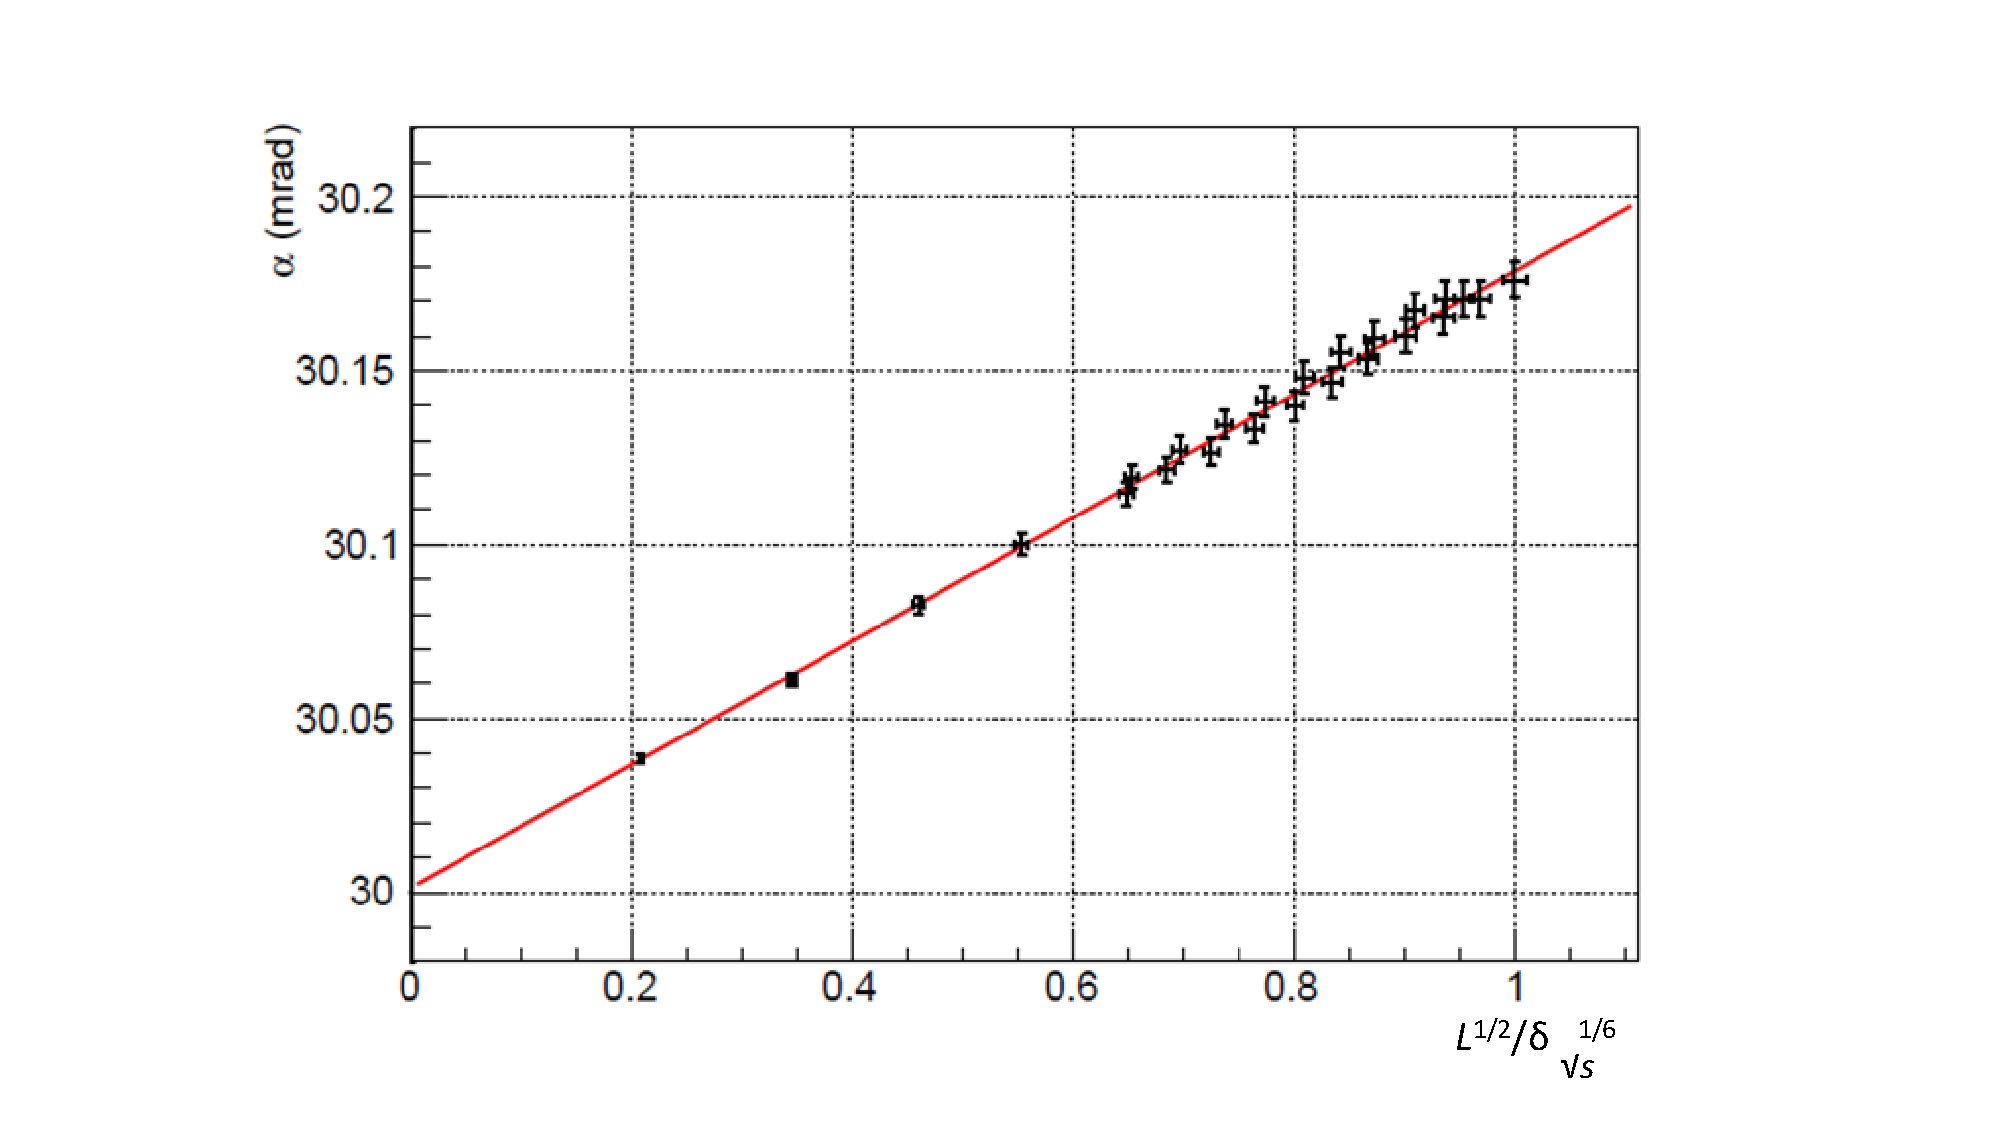
\includegraphics[width=0.75\linewidth]{Physics/EnergyCalibrationPolarisationMonochromatisation/Figs/alpha_kick.pdf}
\caption{Change in the measured crossing-angle $\alpha$ vs.\ $\mathcal{L}^{1/2} \,/\, {\delta_{\sqrts}}^{1/6}$, at various points during the top-up injection.
Extrapolation down to $\mathcal{L}^{1/2} \,/\, {\delta_{\sqrts}}^{1/6}=0$ allows the crossing-angle to be determined in the absence of bunch-bunch effects~\cite{Blondel:2019jmp}.} 
\label{fig:alphakick}
\end{figure}
    
\subsubsection{The longitudinal boost and the collision-energy spread}

The dimuon topology allows the longitudinal boost to be determined on an event-by-event basis.  
When averaged over a suitable sample size, this provides invaluable information to constrain the model of the energy loss around the ring and to calculate the local collision energy at each interaction point.  
The width of this distribution (Fig.~\ref{fig:ecmspread}) is a measure of $\delta_{\sqrts}$, which is an essential input to the measurement of certain observables, such as the \PZ and \PW widths. 
Again, the foreseen statistical precision on these quantities is excellent. 
For example, the energy spread can be measured to one part in a thousand with one million dimuon events.   
Recent work~\cite{delta-sqrts-ISR-corrections}
has investigated how sensitive the determination of $\delta_{\sqrts}$ is to the knowledge of the ISR corrections in dimuon production.  
The conclusion is that the measurement is robust; even if it is assumed that the second-order corrections from ISR are unknown (which is not the case), the resulting bias on the extraction of $\delta_{\sqrts}$ is far smaller than the statistical uncertainty.

\begin{figure}[ht]
\centering
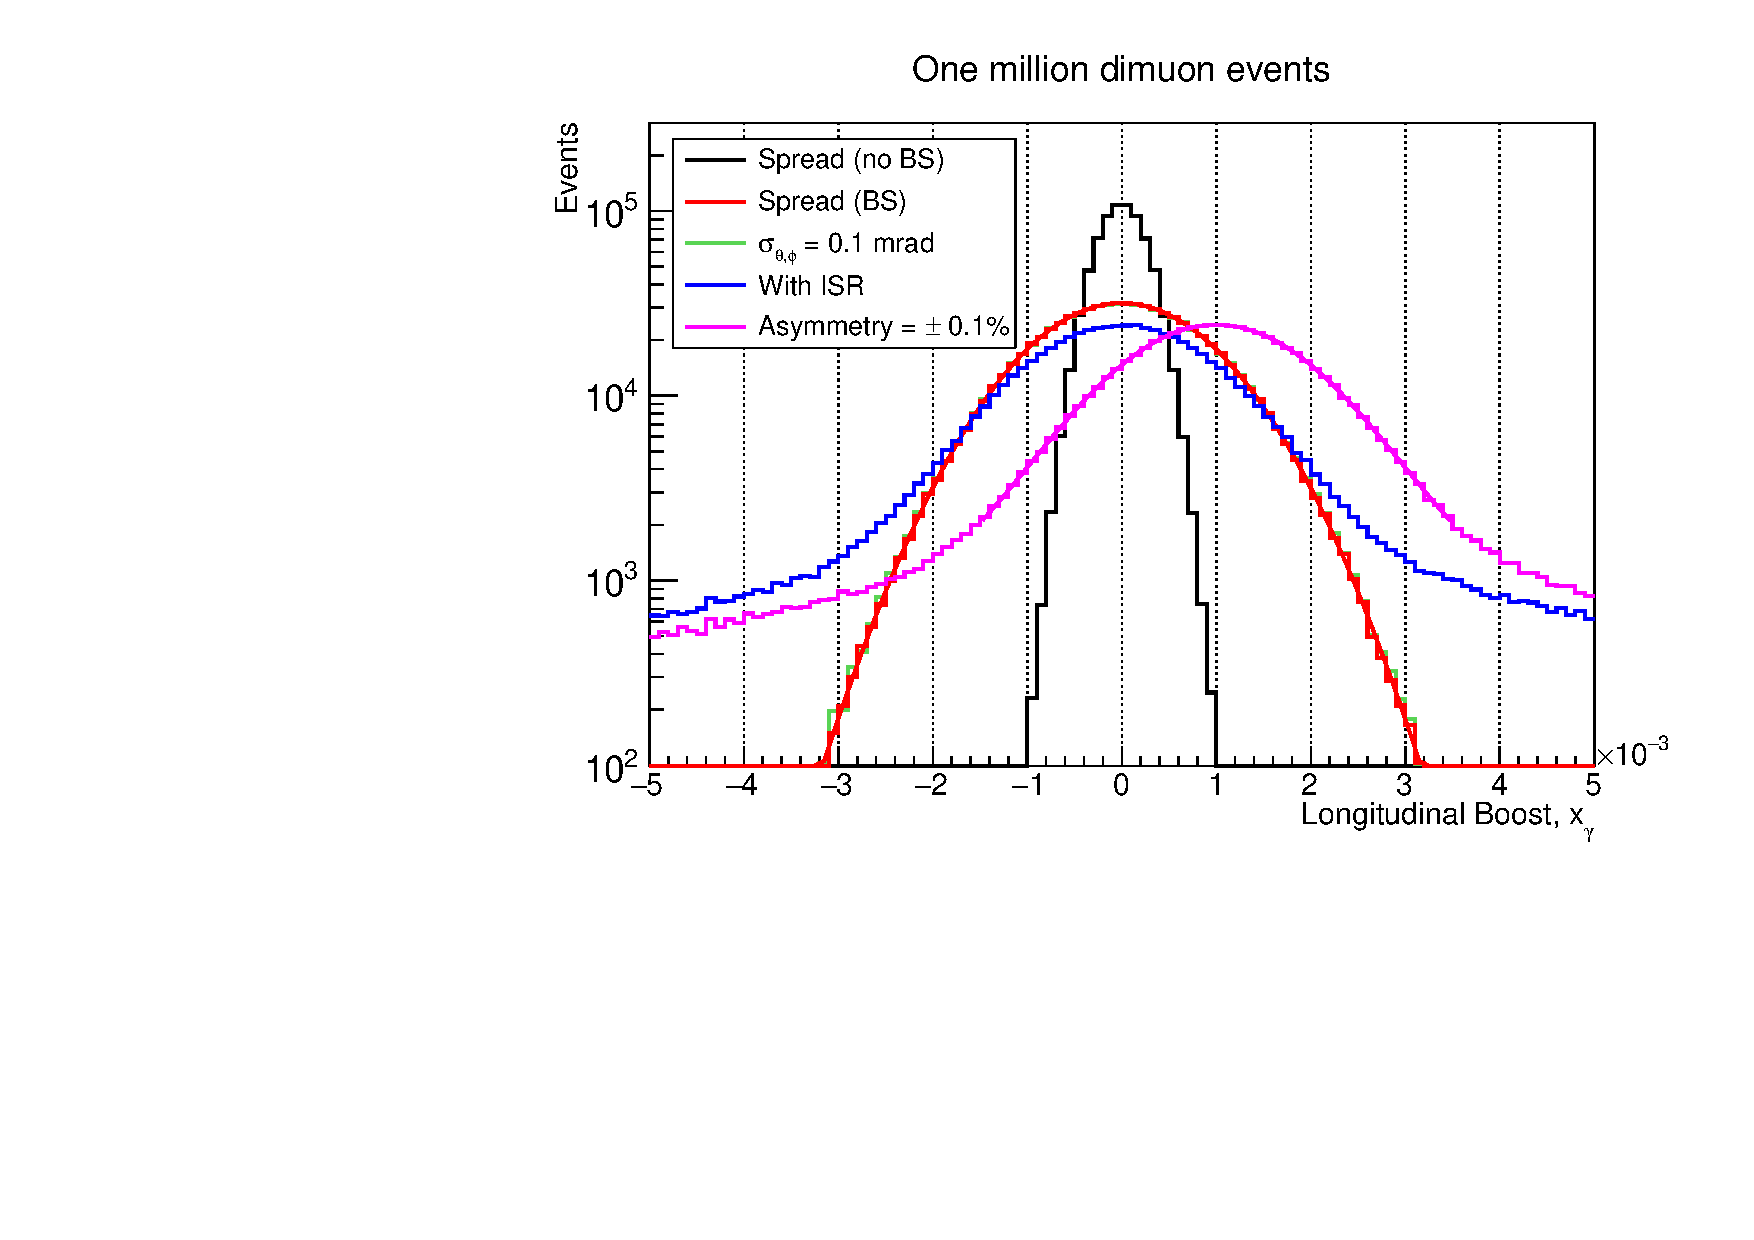
\includegraphics[width=0.7\linewidth]{Physics/EnergyCalibrationPolarisationMonochromatisation/Figs/EnergySpread_Boost-from-EPOL1.pdf} 
\caption{Fitted value of longitudinal boost from one million dimuon events at one of the FCC-ee IPs~\cite{Blondel:2019jmp}. 
Once the ISR is unfolded, this distribution can be used to measure the energy spread. 
The magenta line shows the impact of a centre-of-mass boost on the distribution. 
The shift can be measured with a statistical precision of 40\,keV.  
The other curves indicate the impact of beamstrahlung, angular resolution on the track directions, and ISR.}
\label{fig:ecmspread}
\end{figure}

\subsubsection{Relative \texorpdfstring{$\sqrts$}{ECM} determination in the \texorpdfstring{\PZ}{Z}-resonance scan}

The reconstructed peak position of the dimuon invariant-mass distribution provides an excellent proxy for the collision energy. 
The difference in this reconstructed position between the points of the \PZ-resonance scan provides a measure of the change in collision energy, 
which is a critical input for several analyses, in particular the measurement of the \PZ boson width. 
The distribution is fitted in bins of the polar angle for back-to-back events.  
An example fit is shown in Fig.~\ref{fig:ecmproxy}~(left).
The statistical precision on this pseudo-$\sqrts$ measurement, when summing the samples from four experiments, is around 20\,keV for each of the two off-peak running points, assuming the momentum resolution of the IDEA detector.
So that the detector does not introduce a bias in the measurement larger than the statistical precision, the momentum scale stability must be controlled at this level. 

The field stability can be tracked with NMR probes and the momentum scale can be directly monitored through the reconstruction of low-mass resonances. 
However, even with a perfect detector, there is a bias in the pseudo-$\sqrts$ measurement in the \PZ resonance scan arising from ISR/FSR effects, 
and from the product of the Breit--Wigner shape of the resonance and the Gaussian distribution of the energy spread of the colliding beams. 
The value of this bias varies by about 8\,MeV when going from $\sqrts = 87.9$ to 94.3\,GeV, as can be seen in Fig.~\ref{fig:ecmproxy}~(right).  
This difference must be corrected for in the measurement, which requires a good understanding of the ISR/FSR effects.   
In a generator-level study, disabling ISR/FSR changes the difference in the bias between the two off-peak points by around 500\,keV.  
Therefore, the theoretical prediction of these ISR/FSR effects to the 1\% level would be sufficient to render their impact negligible for the \PZ-width measurement. 

\begin{figure}[t]
\centering
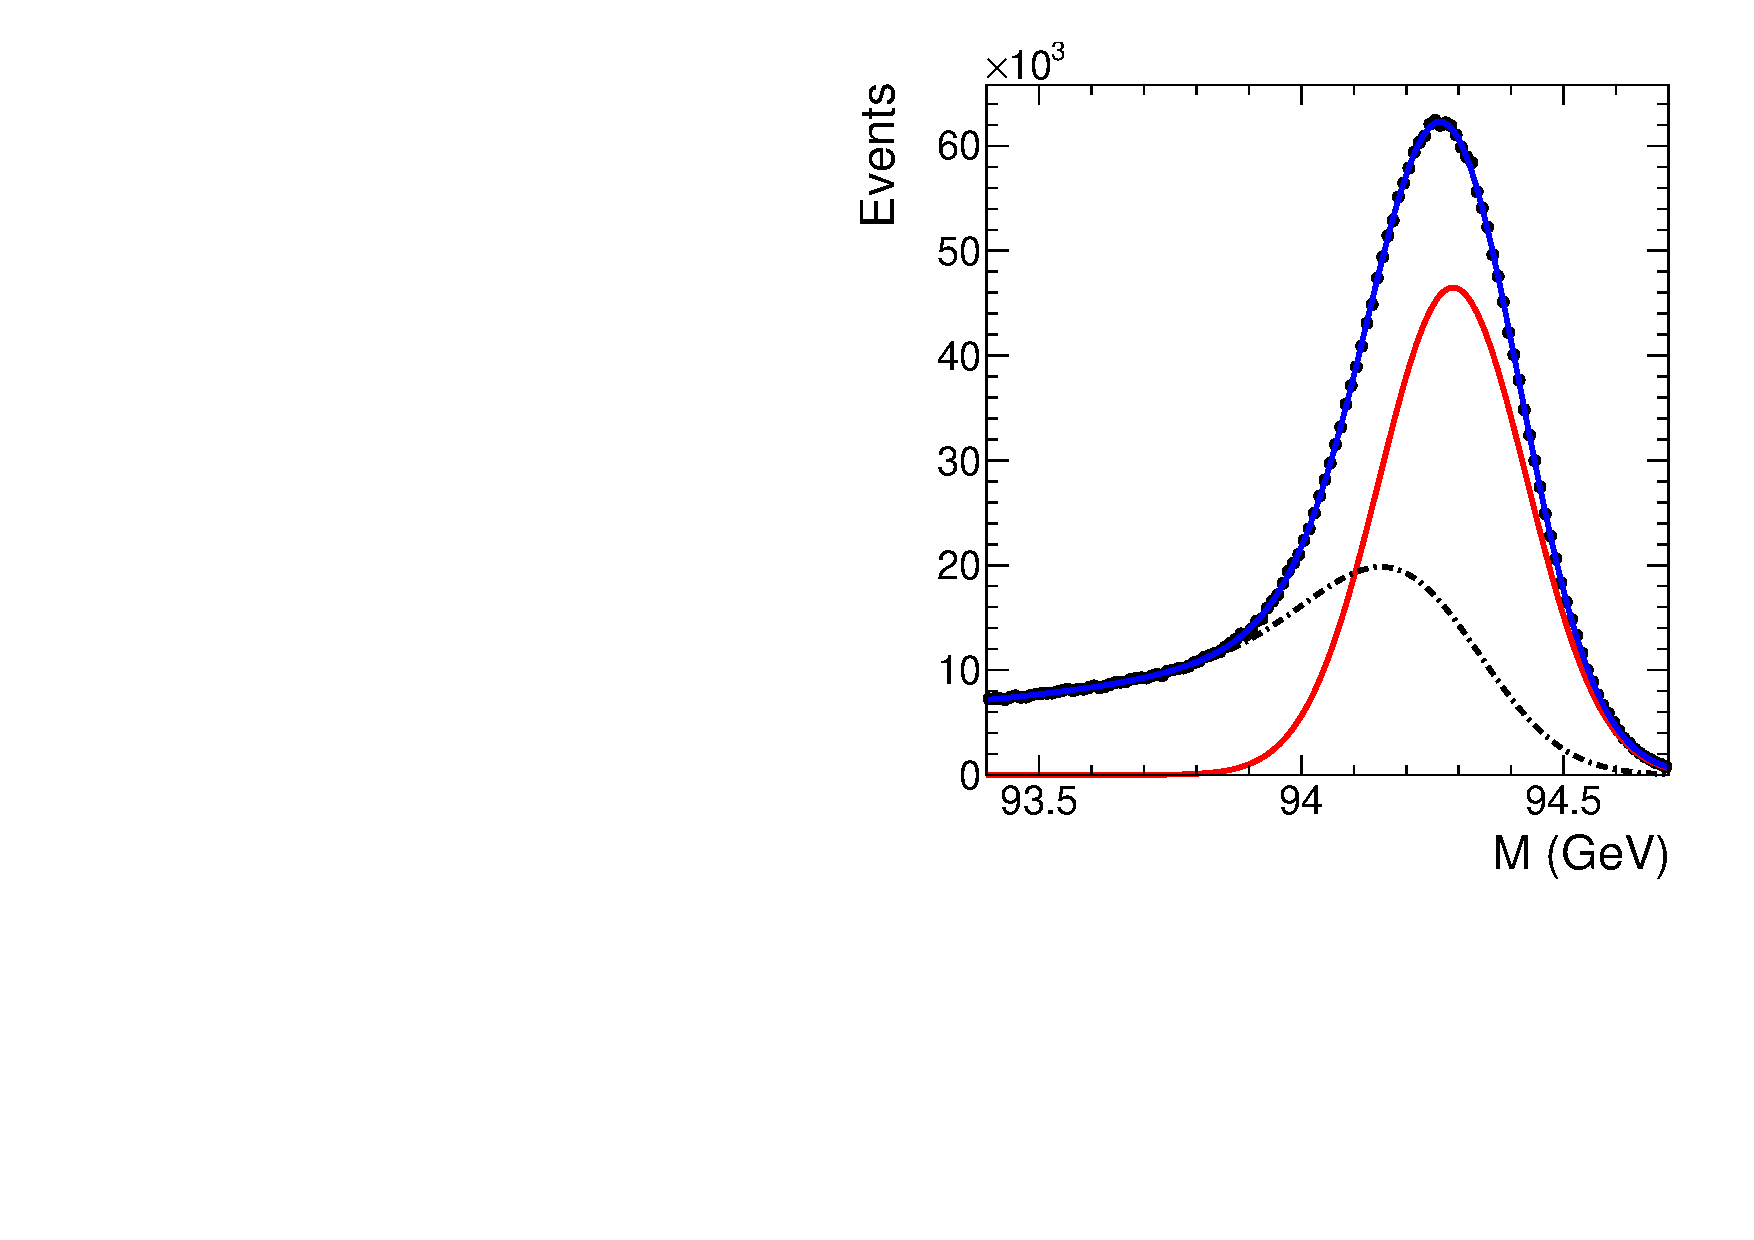
\includegraphics[width=0.49\linewidth]{Physics/EnergyCalibrationPolarisationMonochromatisation/Figs/sqrts_from_dimuons_example_fit.pdf} 
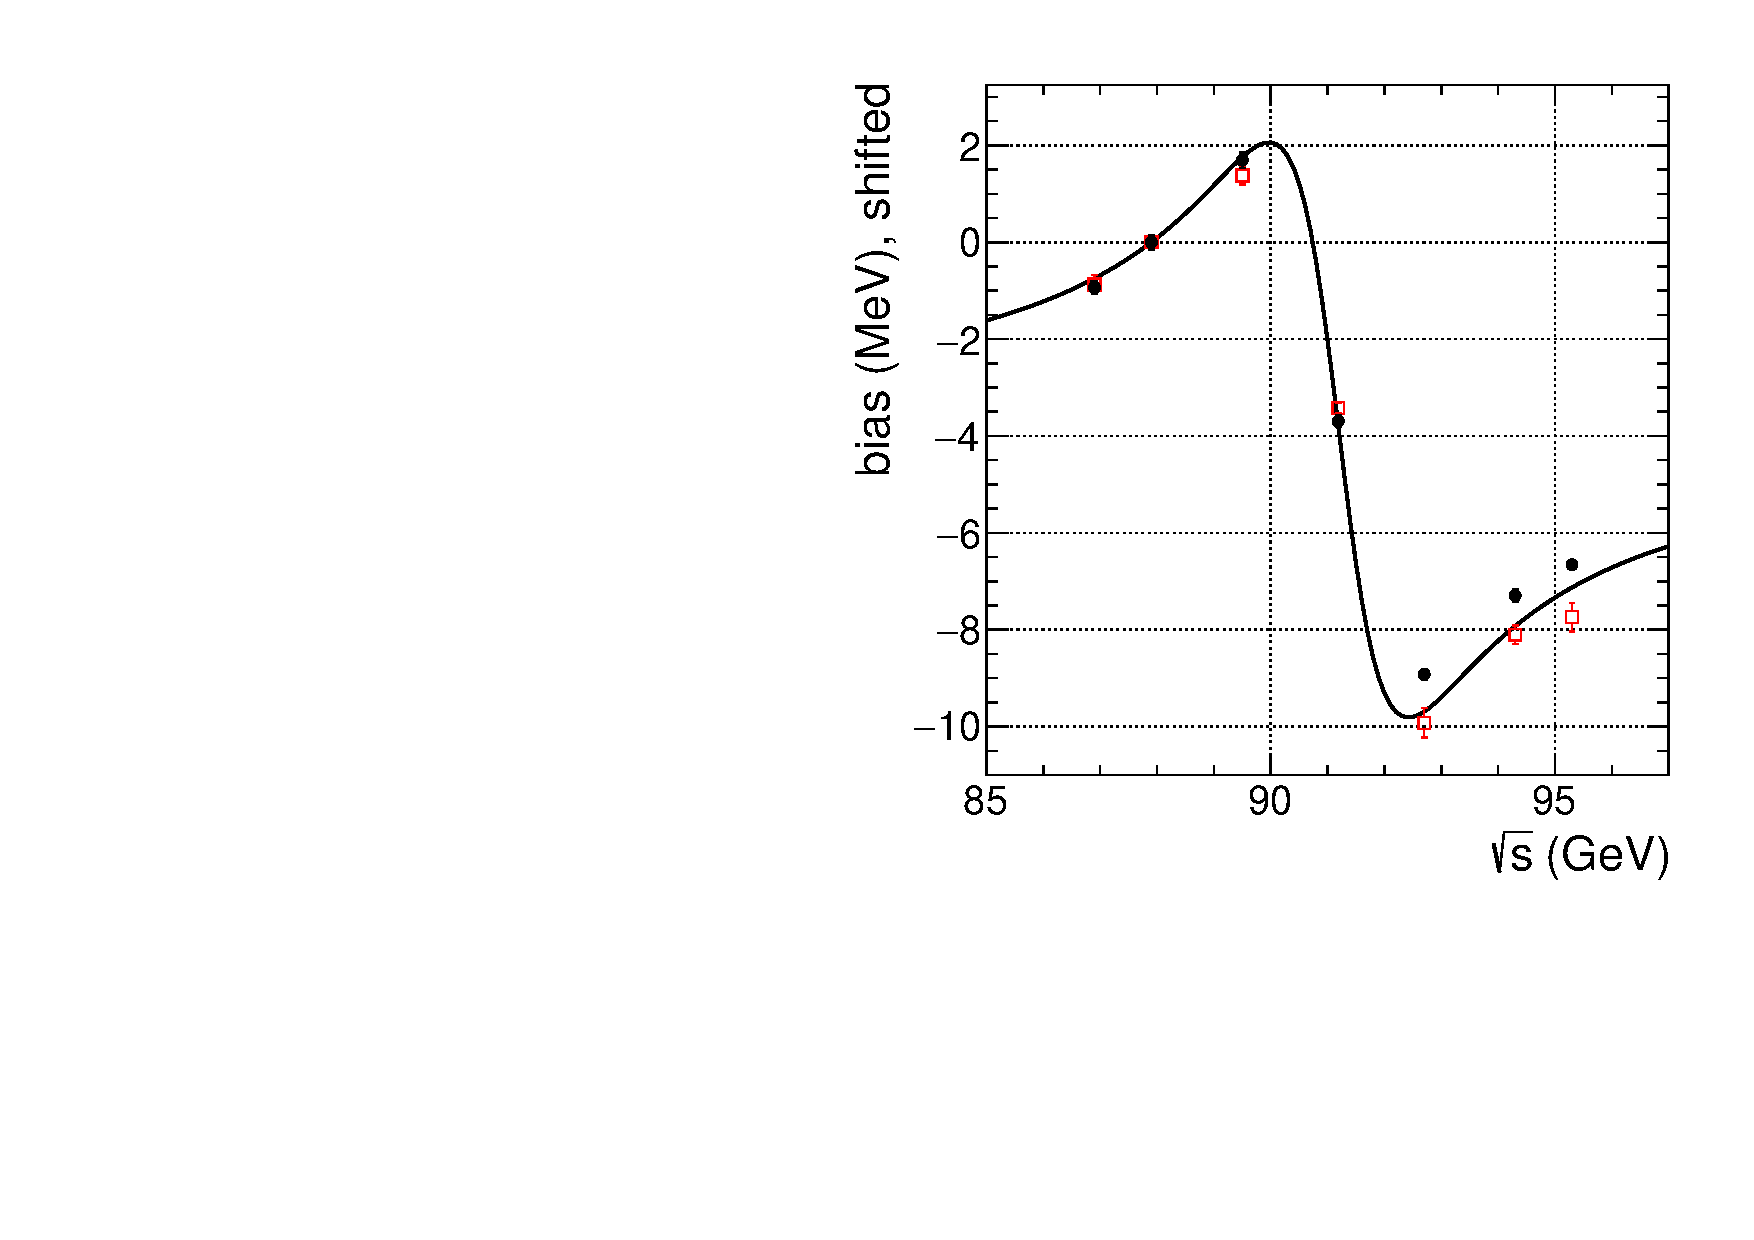
\includegraphics[width=0.49\linewidth]{Physics/EnergyCalibrationPolarisationMonochromatisation/Figs/sqrts_from_dimuons_relativeBias_vs_sqrts.pdf} 
\caption{Left: Example fit to the dimuon invariant-mass distribution at $\sqrts = 94.3$\,GeV, where the peak is modelled with the superposition (blue) of a Gaussian function (red) and two exponential functions (black).  
Right: The difference (bias) between the $\sqrts$ extracted from the dimuon invariant-mass fit and the true value.  
Results are shown for the simulated performance of the IDEA detector (red points) and for the expected dependence, including (black points) or not (black curve) ISR/FSR effects.  
Each set of results also has an overall overset of a few MeV, which is energy independent and, hence, not relevant for the determination of the \PZ width. 
A single shift has been applied to the bias, to correct for these offsets, so that the bias is zero at 87.9\,GeV, for all sets of results.}
\label{fig:ecmproxy}
\end{figure}

\subsubsection{Absolute \texorpdfstring{$\sqrts$}{ECM} determination}

At collision energies above the \PZ boson mass, the dimuon events may be used to provide an absolute measurement of $\sqrts$. 
Radiative returns, in which the emission of an initial-state photon means that the dimuon has the \PZ mass, allows for the calibration of events unaffected by ISR. 
The method can be extended to also include multihadron final states.  
This method can be calibrated at the \PW-pair production threshold with RDP, 
and is of great value for physics studies in the regime where no RDP is possible, 
i.e., collision energies above 200\,GeV. 
This approach also provides a useful complementary measurement of $\sqrts$ in the intermediate energies where RDP is possible but challenging. 
The foreseen statistical uncertainty is 
around 280\,keV for 6\,ab$^{-1}$ of integrated luminosity at $\sqrts = 125$\,GeV 
and 260\,keV for 20\,ab$^{-1}$ at $\sqrts = 160$\,GeV.
The performance of the tracking system must be sufficiently good that the precision is not compromised.

\subsection{Expected precision on EW observables from the collision energy and its spread}

Several of the most important electroweak observables are expected to have a dominant or significant systematic uncertainty associated with the knowledge of the collision energy and collision-energy spread.   
The collision-energy uncertainties can be classed in three distinct categories, itemised below.  
These uncertainties propagate to the physics results in an observable-dependent manner, as discussed in Ref.~\cite{Blondel:2019jmp}.

\begin{itemize}
    \item  Uncertainties that are fully correlated between measurements propagate to the knowledge of the absolute energy scale.  
    Examples include the values of the anomalous magnetic moment and the mass of the electron, the frequency of the RF system, and any other systematic bias that occurs at all times and all energies.  
    At this stage in the studies, it is estimated that this uncertainty will be around 100\,keV on the collision energy at the \PZ pole and 300\,keV at the $\PW^+\PW^-$ threshold.  
    This contribution is expected to be the dominant systematic uncertainty in the measurements of the \PZ and \PW boson masses.
%
    \item A point-to-point contribution comprises biases that occur at all times, or lead to an average shift, but are different for each energy setting.  
    The principal method of determining this uncertainty will be based on the dimuon invariant-mass distribution, as reconstructed by the experiments.  
    The estimated magnitude of this uncorrelated uncertainty is 20\,keV for each off-peak point of the \mbox{\PZ-resonance} scan.  
    The understanding gained at the \PZ pole and complementary measurements will lead to a corresponding uncertainty of around 100\,keV at the $\PW^+\PW^-$ threshold.  
    The point-to-point uncertainty is expected to be the dominant contribution in the measurement of the \PZ width.
%
   \item The uncertainty on each individual RDP measurement is dominated by an uncertainty that is set by the frequency of the polarimeter sampling or the size of the energy bins where the depolarisation can be located.  
   A reasonable estimate of this uncertainty is 200\,keV at the \PZ pole and 300\,keV  at the $\PW^+\PW^-$ threshold.   
   As this component is statistical in nature, its impact decreases with the square-root of the number of events. 
   As it is planned to collect $\sim$\,$10^4$ measurements at each energy point, the final uncertainty from this source will be essentially negligible, compared to other contributions.  
   However, the importance of making each measurement as precise as possible, and of collecting the largest possible number of measurements, will become more evident when the data set is split into smaller samples to perform systematic checks.
\end{itemize}

\begin{table}[h]
\centering
\caption{Current projected $\sqrts$-related uncertainties on selected electroweak observables.}  
\label{tab:DS-Ecal-errors-final}
\begin{tabular}{cccccc} \toprule
    & \multicolumn{5}{c}{Observable} \\
    Uncertainty 
    & $m_{\PZ}$ (keV) & $\Gamma_{\PZ}$ (keV) 
    &  $\sin^2 \theta^\text{eff}_{\PW}$ ($\times 10^{-6}$) 
    & $\frac{\Delta \alpha_\text{QED}(m^2_{\PZ})}{\alpha_\text{QED}(m^2_{\PZ})}$ ($\times 10^{-5}$) 
    & $m_{\PW}$ (keV) \\ 
\midrule
    Absolute & 100 & 2.5 & -- & 0.1 & 150 \\
    Point-to-point & 14 & 11 & 1.2 & 0.5 & 50 \\
    Sample size & 1 & 1 & 0.1 & -- & 3 \\
    Energy spread & -- & 5 & -- & 0.1 & -- \\ 
\midrule
    Total $\sqrts$-related & 101 & 12 & 1.2 & 0.5 & 158 \\ 
\midrule
    FCC-ee statistical & 4 & 4 & 1.2 & 3.9 & 180 \\  
\bottomrule
\end{tabular}
\end{table}

The contributions from each uncertainty category, and their quadratic sum, are listed in Table~\ref{tab:DS-Ecal-errors-final} for several key electroweak observables.
This table also shows the contribution from the uncertainty in the knowledge of the energy spread, which affects quantities with a strong quadratic dependence on the collision energy.  
Observables that are most susceptible to this uncertainty include the \PZ cross section and the \PZ width.  
A collision-energy spread of 70\,MeV, determined with a precision of $\pm$\,0.05\,MeV, leads to a sub-dominant systematic uncertainty in the measurement of these observables.

With the current expectations, it will be possible to reduce the uncertainty from energy-related quantities by an order of magnitude or more with respect to what was achieved at LEP, such that they will be smaller than, or similar to, the statistical uncertainty for all observables apart from $m_{\PZ}$.  
Indeed, the entries in Table~\ref{tab:DS-Ecal-errors-final} for the $\sqrts$-related systematic uncertainties can be compared to the corresponding LEP values of 
1.7\,MeV for $m_{\PZ}$, 1.2\,MeV for $\Gamma_{\PZ}$, and 9\,MeV for $m_{\PW}$. 

\subsection{Prospects for monochromatisation and the measurement of the electron Yukawa coupling}
\label{sec:eYukawa}

This section describes the tantalising possibility, unique to FCC-ee, 
to observe the $s$-channel process $\Pep\Pem \to \PH$, and thereby determine the electron Yukawa coupling.  
The challenges are very demanding and progress is required from both the accelerator and the experimental analyses, but the current studies, described below, are encouraging.

\subsubsection*{The electron Yukawa via resonant Higgs production at 125\,GeV}

Confirming the mechanism of mass generation for the stable visible elementary particles of the universe, 
composed of $\PQu$ and $\PQd$ quarks plus the electron (and neutrinos), 
is experimentally very challenging because of the low masses of the first-generation fermions and, thereby, 
their small Yukawa couplings to the Higgs field. (The neutrino mass generation remains a BSM problem in itself.) 
In the SM, the Yukawa coupling of the electron is $y_{\Pe} = \sqrt{2} \, m_{\Pe}/v = 2.8 \cdot 10^{-6}$, 
for $m_{\Pe}(m_{\PH}) = 486$\,keV and Higgs vacuum expectation value $v = ( \sqrt{2} \, G_\mathrm{F} )^{-1/2} = 246.22$\,GeV.
Measuring it via $\PH \to \Pep\Pem$ appears hopeless at hadron colliders because the decay has a tiny partial width, 
proportional to the electron mass squared,
\begin{equation}
\Gamma(\PH\to\Pep\Pem) = 
\frac{{G_\mathrm{F}} \, m_{\PH} \, m_{\Pe}^2} {4\,\sqrt{2}\,\pi}
\left(1-\frac{4\,m^2_{\Pe}}{m^2_{\PH}}\right)^{3/2} = 2.14 \times 10^{-11} \, \text{GeV} \, ,
\label{eq:Gamma_H_ee}
\end{equation}
which corresponds to a branching fraction $\mathcal{B}(\PH\to\Pep\Pem) \approx 5 \times 10^{-9}$ 
for the SM Higgs boson. 
At LHC and FCC-hh, such a final state is completely swamped by the Drell--Yan $\Pep\Pem$ continuum. 
The current LHC searches~\cite{ATLAS:2019old,CMS:2022urr}, 
exploiting about 140\,fb$^{-1}$ of pp data at $\sqrts = 13$\,TeV,
reach an observed upper limit on the branching fraction 
of $\mathcal{B}(\PH\to\Pep\Pem) < 3.0 \times 10^{-4}$ at 95\% CL. 
This value translates into the current upper bound on the Higgs boson effective coupling modifier to electrons of $\lvert \kappa_{\Pe} \rvert  < 240$. 
Assuming that the sensitivity to the $\PH \to \Pep\Pem$ decay scales simply with the square root of the integrated luminosity, 
the HL-LHC phase with a $\LumiInt = 2\times 3$\,ab$^{-1}$ data sample 
(combining the ATLAS and CMS results) 
will result in $y_{\Pe} \lesssim 100 ~ y^\mathrm{\textsc{sm}}_{\Pe}$. 
Based on searches for the similar $\PH \to \PGmp\PGmm$ channel, 
one can expect upper limits on $\mathcal{B}(\PH\to\Pep\Pem)$ to be further improved by factors of about four, 
by adding more Higgs production categories and using advanced multivariate analysis methods, 
eventually reaching $y_{\Pe} \lesssim 50 ~ y^\mathrm{\textsc{sm}}_{\Pe}$ at the end of the HL-LHC.

About ten years ago, it was first noticed that the unparalleled integrated luminosities 
of $\LumiInt \approx 10$\,ab$^{-1}$/year expected at $\sqrts = 125$\,GeV at the FCC-ee 
would make it possible to attempt an observation of the direct production of the scalar boson and, thereby, 
a direct measurement of the electron Yukawa coupling~\cite{dEnterria:2014,dEnterria:2017dac}. 
Subsequently, several 
theoretical studies~\cite{Jadach:2015cwa,Greco:2016izi,Dery:2017axi,Davoudiasl:2023huk,Boughezal:2024yjk}, 
simulated data analysis~\cite{dEnterria:2021xij}, 
and accelerator studies~\cite{Zimmermann:2017tjv,telnov2020monochromatizationeecolliderslarge,Faus-Golfe:2021udx} 
have explored the various aspects connected to the $\Pep\Pem\to\PH$ measurement. 

The Feynman diagrams for $s$-channel Higgs production 
(and its statistically most significant decay at FCC-ee, $\PH \to \Pg\Pg$, see below) 
and dominant backgrounds are shown in Fig.~\ref{fig:eeH_diags}~(left). 
The resonant Higgs cross section in $\Pep\Pem$ collisions as a function of $\sqrts$ 
is theoretically given at Born level by the relativistic Breit--Wigner (BW) expression:
\begin{equation}
\sigma_{\Pe\Pe \to \PH} = \frac{4\, \pi\, \Gamma_{\PH}\, \Gamma(\PH\to\Pep\Pem)} {(s-m_{\PH}^2)^2 + m_{\PH}^2\Gamma_{\PH}^2} \, .
\label{eq:sigma_H_ee}
\end{equation}
An accurate knowledge of $m_{\PH}$ is, therefore, critical to maximise the resonant cross section. 
An $\cal{O}$(4\,MeV) precision on the Higgs boson mass can be achieved (Section~\ref{sec:ch_part_tracking}) before any dedicated $\Pep\Pem\to\PH$ run.
In addition,  the FCC-ee beam energies will be monitored with a relative precision of $10^{-6}$, providing a sub-MeV accuracy on the exact point in the Higgs lineshape being probed at any moment.

\begin{figure}[t]
\centering

\includegraphics[width=0.27\columnwidth]{Physics/EnergyCalibrationPolarisationMonochromatisation/Figs/feynam_diags_eeH.png}
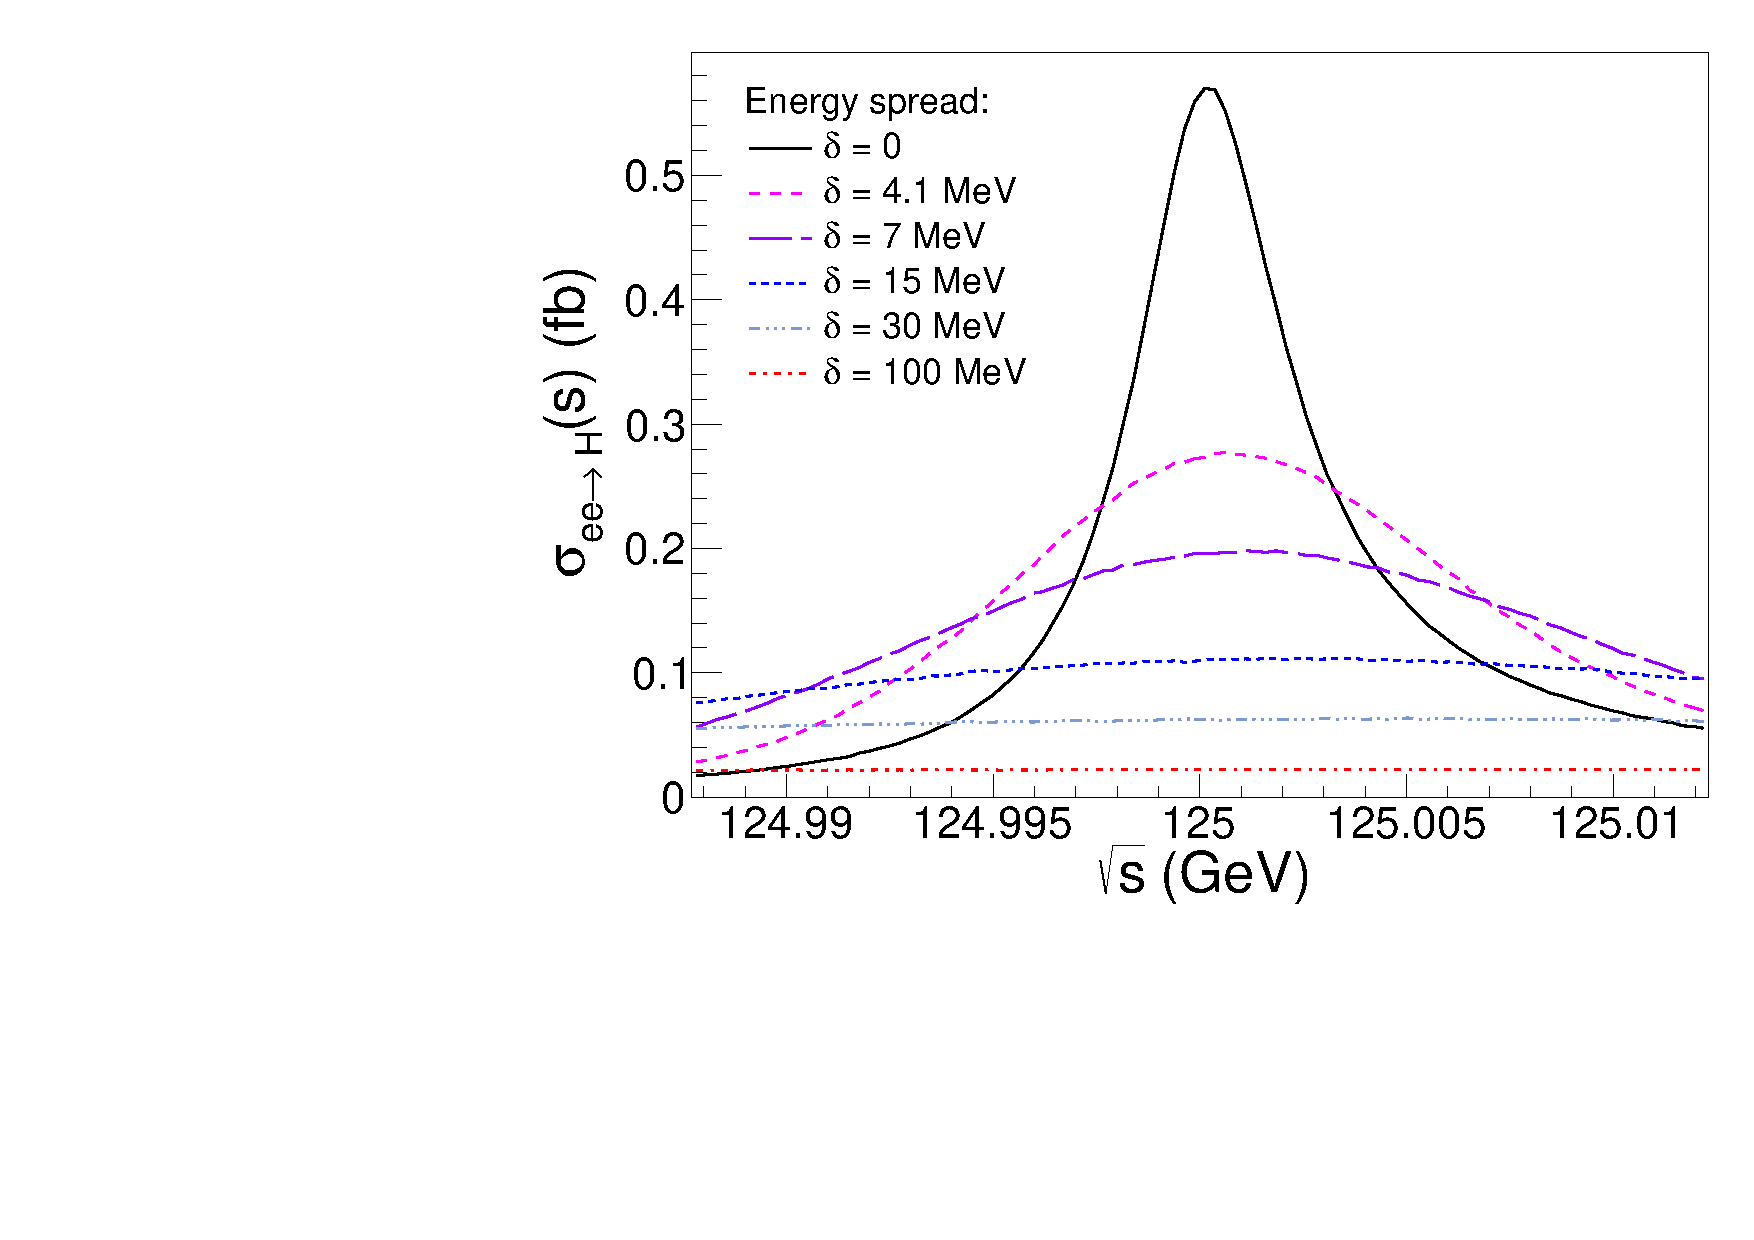
\includegraphics[width=0.53\columnwidth]{Physics/EnergyCalibrationPolarisationMonochromatisation/Figs/BW_Higgs_ISR_spread.pdf}
\caption{Left: Diagrams for the $s$-channel production of the Higgs boson decaying into two gluon jets (top) 
and reducible $\PZ^*$ quark dijet backgrounds (bottom) in $\Pep\Pem$ at $\sqrts = 125$\,GeV. 
Right: Resonant Higgs production cross section at $\sqrts = 125$\,GeV, including ISR effects, 
for several $\Pep\Pem$ collision energy spread values: $\delta_{\sqrts} = 0$, 4.1, 7, 15, 30, and 100\,MeV~\cite{Jadach:2015cwa}.
\label{fig:eeH_diags}}
\end{figure}

For $m_{\PH} = 125$\,GeV, Eq.~\ref{eq:sigma_H_ee} gives 
$\sigma_{\Pe\Pe \to \PH} = 4\,\pi\,\mathcal{B}(\PH\to\Pep\Pem) / m_{\PH}^2 = 1.64$\,fb as peak cross section. 
Two effects, however, lead to a significant reduction of the Born-level prediction: 
(i)~ISR depletes the cross section and generates an asymmetry of the Higgs lineshape; and 
(ii)~the actual beams are never perfectly monoenergetic, i.e., 
the collision $\sqrts$ has a spread $\delta_{\sqrts}$ around its central value,
further leading to a smearing of the BW peak. 
For FCC-ee operating at 125\,GeV, 
the natural spread in collision energy due to synchrotron radiation will be around 70\,MeV. 
Monochromatisation aims at reducing $\delta_{\sqrts}$ to the few MeV scale, while still delivering moderately large (few ab$^{-1}$) integrated luminosities, $\LumiInt$~\cite{Zimmermann:2017tjv,telnov2020monochromatizationeecolliderslarge,Faus-Golfe:2021udx}. 
The reduction of the BW cross section due to  initial-state photon emission(s) alone 
is of a factor of 0.35 and leads to $\sigma_{\Pe\Pe \to \PH} = 0.57$\,fb~\cite{Jadach:2015cwa}. 

The additional impact of a given energy spread on the Higgs BW shape can be quantified through the convolution of BW and Gaussian distributions, i.e., a relativistic Voigtian function. 
Figure~\ref{fig:eeH_diags}~(right) shows the Higgs lineshape for various $\delta_{\sqrts}$ values. 
The combination of ISR plus $\delta_{\sqrts} = \Gamma_{\PH} = 4.1$\,MeV reduces the peak Higgs cross section by a total factor of 0.17, 
down to $\sigma_{\Pe\Pe \to \PH} = 0.28$\,fb. 
Though tiny, the cross section for any other $\Pep\Pem \to \PH$ production process, through intermediate \PW or \PZ bosons, 
is much further suppressed by the electron mass for on-shell external fermions (chirality flip)~\cite{Altmannshofer:2015qra} 
and is negligible as well as any other loop-induced Higgs production mechanisms at $\sqrts = 125$\,GeV 
that is not sensitive to $y_{\Pe}$~\cite{DdE_Dung2025}.

The strategy to observe the resonant production of the Higgs boson~\cite{dEnterria:2021xij} 
is based on identifying final states consistent with any of the \PH decay modes 
that lead to small (but statistically significant when combined together) excesses over the expected backgrounds  
(orders-of-magnitude more abundant than the signal). 
In Ref.~\cite{dEnterria:2021xij}, a detailed study was performed with large simulated event samples of signal 
and associated backgrounds generated with \pythia~8~\cite{pythia8} for eleven Higgs boson decay channels. 
A benchmark monochromatisation point of $(\delta_{\sqrts},\LumiInt)=(4.1\,\text{MeV},10\,\text{ab}^{-1})$, 
corresponding to 2800 Higgs bosons produced, was assumed for the signal. 
A simplified description of the expected experimental performance was considered for the reconstruction and (mis)tagging 
of heavy-quark ($\PQc$, $\PQb$), light-quark ($\PQu\PQd\PQs$), and gluon ($\Pg$) jets, as well as photons, electrons, and hadronically decaying tau leptons. 
Generic preselection criteria were defined to suppress reducible backgrounds while keeping the largest fraction of the signal events. 
A subsequent multivariate analysis of $\cal{O}$(50) kinematic and global topological variables, defined for each event, was carried out. 
Boosted Decision Tree (BDT) classifiers were trained on signal and background events to maximise the signal significance for each individual channel. 
The most significant Higgs decay channels are found to be $\PH \to \Pg\Pg$ 
(for a gluon efficiency of 70\% and a $\PQu\PQd\PQs$-for-$\Pg$ jet mistagging rate of 1\%), 
and $\PH\to\PW\PW^* \to \ell\,\PGn\,jj$. 
The digluon final state is the most sensitive channel to search for the resonant Higgs boson production (Fig.~\ref{fig:eeH_diags}~left, upper diagram) because it has a moderately large branching fraction ($\mathcal{B}\approx 8\%$) 
while the $\PZ^*\to\Pg\Pg$ decay is forbidden by the Landau--Yang theorem. 
The most important experimental challenge is to reduce the light-quark for gluon mistagging rate to the 1\% level 
(while maintaining the efficiency for the $\PH\to\Pg\Pg$ channel at 70\%) 
to keep the overwhelming $\PZ^*\to \uubar$, $\ddbar$, $\ssbar$ backgrounds (Fig.~\ref{fig:eeH_diags}~left, lower diagram) under control. 
Such a mistagging rate is a factor of about seven times better than the current state-of-the-art for jet-flavour tagging algorithms~\cite{Bedeschi:2022rnj}, 
but it is a realistic goal given all the experimental and theoretical improvements in the understanding of parton radiation and hadronisation expected at the FCC-ee~\cite{Proceedings:2017ocd}.

Combining all results for an accelerator operating at $(\delta_{\sqrts},\LumiInt)=(4.1\,\text{MeV},10\,\text{ab}^{-1})$, 
a 1.3\,$\sigma$ signal significance can be reached for the direct production of the Higgs boson, 
corresponding to an upper limit on the electron Yukawa coupling at 1.6 times the SM value: 
$\lvert y_{\Pe} \rvert < 1.6 \, \lvert y^\mathrm{\textsc{sm}}_{\Pe} \rvert $ at 95\% CL for each detector in one  year. 
Based on this benchmark result and the dependence of the resonant Higgs cross section on $\delta_{\sqrts}$ 
(Fig.~\ref{fig:eeH_diags}, right), 
bidimensional maps of $\Pep\Pem\to\PH$ significance and electron-Yukawa sensitivities have been determined in the $(\delta_{\sqrts},\LumiInt)$ plane. 

\begin{figure}[ht]
\centering

\includegraphics[width=0.65\textwidth]{Physics/EnergyCalibrationPolarisationMonochromatisation/Figs/eeH_eYukawa_limits_2024_without_crab.png}
\caption{Upper limit contours (at 95\% CL) on the electron Yukawa $y_{\Pe}$ (coloured bands) 
in the collision-energy spread $\delta_{\sqrts}$ vs.\ integrated luminosity $\LumiInt$ plane.
The red star over the $\delta_{\sqrts} = \Gamma_{\PH} =4.1$\,MeV red-dashed line indicates the reference point assumed in the physics simulation analysis~\cite{dEnterria:2021xij}. 
The black cross indicates the previously achieved working point with self-consistent parametric monochromatisation~\cite{ValdiviaGarcia:2022nks,Faus-Golfe:2021udx}.
The red and yellow squares indicate the monochromatisation points based on simulations of the `GHC V22 Z' and `GHC V22 $\PQt\PAQt$' optics, respectively 
(see text for details)~\cite{Zhang:2024sao}.
\label{fig:eeH_signif}}
\end{figure}

Figure~\ref{fig:eeH_signif} shows the 95\% CL upper limit contours on the electron Yukawa coupling strength as a function of the energy spread and integrated luminosity with the red star 
(on the red-dashed line corresponding to a reference monochromatised collision-energy spread equal to the Higgs boson width), 
indicating the result of this benchmark study. 
The next section discusses the results of the current monochromatisation simulation studies, shown with red and yellow squares in this figure.

\subsubsection*{FCC-ee monochromatisation}
Monochromatisation is necessary to reduce 
$\delta_{\sqrts}$ to the few MeV level of the natural SM Higgs width and thereby increase the sensitivity of the electron-Yukawa measurement via $\Pep\Pem \to \PH$. 
This strategy was first proposed 50 years ago~\cite{Renieri:1975wt} and relies on creating opposite correlations between spatial position and energy deviations within the colliding beams with nominal beam energy $E_0$. 
Figure~\ref{fig:monochromschem} shows a schematic of the principle of monochromatisation for beams that collide head on (left) and with a crossing angle $\alpha$ (right).  
The current baseline design of FCC-ee corresponds to the latter configuration. 
In both configurations, the correlations between transverse (either horizontal or vertical) position in the beam and energy lead to a lower spread in collision energy than in the uncorrelated case.

\begin{figure}[ht]
\centering
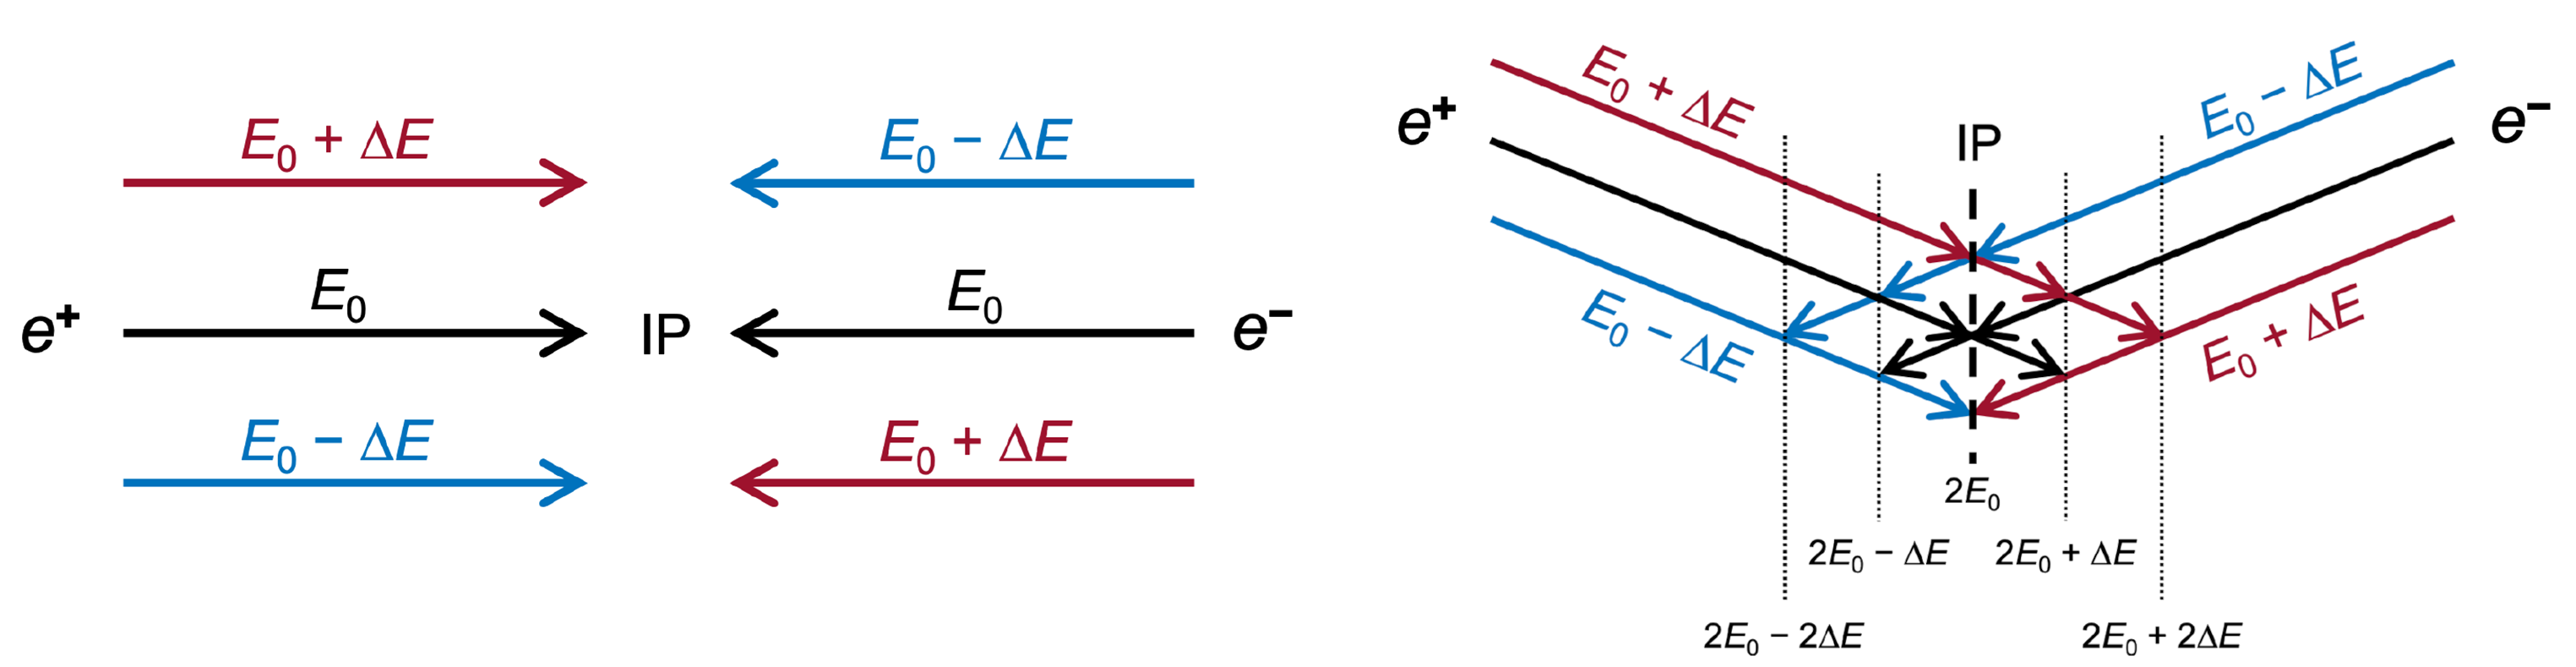
\includegraphics[width=0.9\textwidth]{Physics/EnergyCalibrationPolarisationMonochromatisation/Figs/monochrom_cartoon2.png}
\caption{Schematic of the principle of monochromatisation for head-on collisions (left) and collisions with a crossing angle (right). 
In both cases, opposite-sign correlations between the transverse position in the beam and the energy lead to a reduction in the collision-energy spread, compared with the uncorrelated case.}
\label{fig:monochromschem}
\end{figure}

Monochromatisation can be achieved by adding dedicated components at the interaction region (IR) to generate a non-zero dispersion function with opposite signs for the two beams at the IP. 
A non-zero dispersion function at the IP in the horizontal and/or vertical directions ($D_{x,y}^{\ast} \neq 0$) enlarges the IP transverse beam size ($\sigma_{x,y}^{\ast}$), which in turn affects the luminosity, $\mathcal{L} \propto 1/(\sigma_{x}^{\ast} \sigma_{y}^{\ast})$. 
The monochromatisation factor is defined as
\begin{equation}
    \lambda = \sqrt{1 + \sigma_{\delta}^2 
    \left( \frac{D_x^{\ast 2}}{\varepsilon_{x} \, \beta_{x}^{\ast}} + \frac{D_y^{\ast 2}}{\varepsilon_{y} \, \beta_{y}^{\ast}} \right) } \, ,
\label{eq:lambda_monochrom}
\end{equation}
where $\sigma_{\delta}$ is the relative energy spread, $\varepsilon_{x,y}$ the transverse emittances, and $\beta_{x,y}^{\ast}$ the betatron functions at the IP. 
For any value of $\lambda$ achieved, $\delta_{\sqrts}$ and $\mathcal{L}$ in the monochromatisation operation mode are
\begin{equation}
    \delta_{\sqrts} = \frac{\sqrt{2} \, E_0 \, \sigma_\delta}{\lambda} \quad \text{and} \quad 
    \mathcal{L} = \frac{\mathcal{L}_0}{\lambda} \, ,
\label{eq:delta_sqrts}
\end{equation}
where $\mathcal{L}_0$ represents the luminosity for the same values of $\beta_{x,y}^{\ast}$ but without $D_{x,y}^{\ast}$. 
Consequently, the design of a monochromatisation scheme requires considering both the IR beam optics and the optimisation of other collider parameters to maintain the highest possible luminosity. 
Possible approaches to monochromatisation for FCC-ee have been studied for several years, starting from self-consistent parametric studies~\cite{ValdiviaGarcia:2016rdg,Zimmermann:2017tjv,Faus-Golfe:2021udx,ValdiviaGarcia:2022nks}. 
Recent  developments~\cite{Zhang:2024sao,Zhang:2024phd} comprise a detailed study of the IP-region optics required for monochromatisation, exploring different potential configurations and their implementation in the FCC-ee global lattice, along with beam-dynamics simulations and performance evaluations including the impact of beamstrahlung. 

The baseline FCC-ee standard lattice design is the so-called `Global Hybrid Correction' (GHC) optics~\cite{Oide:2016mkm,Keintzel:2023myn,vanRiesen-Haupt:2024ore}.
It allows for four IRs, where the $\Pep$ and $\Pem$ beams are brought to collision 
with an $\alpha= 30$\,mrad angle in the horizontal plane, as well as a potential vertical crab-waist scheme. 
The results of the monochromatisation studies shown in Fig.~\ref{fig:eeH_signif} are based on two versions of this optics: 
`GHC V22 Z', where the lattice is optimised for operation at the \PZ pole, and 
`GHC V22 $\PQt\PAQt$', which is optimised for operation above the $\PQt\PAQt$ threshold 
(in both, `V22' designates the 2022 configuration).
Three approaches to monochromatisation have been investigated.  
In the first, the horizontal dipoles used for the local-chromaticity-correction system are reconfigured to generate a non-zero $D^\ast_x$ of size ${\sim}\, 10$\,cm, 
while maintaining the same $\alpha$ value.  
Given the values of the other parameters in Eq.~(\ref{eq:lambda_monochrom})~\cite{Keintzel:2023myn}, it follows that monochromatisation factors in the range $\lambda = 5$--8 are achievable. 

This study was performed both to provide monochromatisation in all four IRs and then repeated to give monochromatisation in only two IRs.
The second method introduces a non-zero value of $D^\ast_y$ by adjusting the strengths of the skew quadrupoles in the interaction region.  
The very low vertical emittance in FCC-ee implies that similar monochromatisation factors as in the horizontal case 
can be achieved with $D^\ast_y \approx 1$\,mm.  
Finally, schemes involving non-zero values of both $D^\ast_x$ and $D^\ast_y$ have been explored.   
In all cases, the layout of the components around the IR and the parameter values were adjusted to satisfy the boundary conditions in the machine and deliver optimum performance.

Simulations were performed with \textsc{Guinea-Pig}~\cite{Schulte:1998au} to determine  the performance of the different monochromatisation schemes, taking into account the impact of beamstrahlung. 
The particle distribution at the IP was simulated as an ideal Gaussian distribution, comprising 40\,000 particles and defined by the following global optical performance parameters: 
$E_0$, $\sigma_{\delta}$, $\varepsilon_{x,y}$, $\beta_{x,y}^{\ast}$, $D_{x,y}^{\ast}$, $\sigma_{z}$, and $\alpha$. 
For each configuration, the $\delta_{\sqrts}$ (from the distribution of the collision energy) and $\mathcal{L}$ were calculated. 
The results are presented in Tables~\ref{tab:monochromZ} and~\ref{tab:monochromtt} for the `GHC V22 Z' and `GHC V22' $\PQt\PAQt$ optics, respectively.
 
\begin{table}[ht]
\caption{Values of $\delta_{\sqrts}$, $\mathcal{L}$, and $\LumiInt$ for five setups of the `GHC V22 Z' monochromatisation IR optics~\cite{Zhang:2024sao}:
without monochromatisation (`Std.\ ZES'), 
with $D^*_x \ne 0$ in four and two IPs (`ZH4IP' and `ZH2IP'),
with $D^*_y \ne 0$ (`ZV'), 
and with $D^*_{x,y} \ne 0$ (`ZHV').}
\label{tab:monochromZ}
\centering
\begin{tabular}{lccccc}\hline
    & Std.\ ZES & ZH4IP & ZH2IP & ZV & ZHV \\\hline
    CM energy spread $\delta_{\sqrts}$ (MeV) & 69.52 & 26.80 & 24.40 & 25.25 & 20.58 \\
    Luminosity / IP $\mathcal{L}$ ($10^{34}$ cm$^{-2}$s$^{-1}$) & 44.8 & 15.0 & 18.4 & 1.46 & 1.42 \\
    Integrated luminosity / IP / year $\LumiInt$ (ab$^{-1}$) & 5.38 & 1.80 & 2.21 & 0.18 & 0.17 \\\hline
\end{tabular}
\end{table}

\begin{table}[ht]
\caption{Same as previous table, but for the `GHC V22 $\PQt\PAQt$' monochromatisation IR optics~\cite{Zhang:2024sao}.}
\label{tab:monochromtt}
\centering
\begin{tabular}{lccccc}\hline
    & Std.\ TES & TH4IP & TH2IP & TV & THV \\\hline
    CM energy spread $\delta_{\sqrts}$ (MeV) & 67.20 & 27.10 & 23.16 & 20.23 & 21.24 \\
    Luminosity / IP $\mathcal{L}$ ($10^{34}$\,cm$^{-2}$s$^{-1}$) & 71.2 & 17.9 & 24.5 & 1.37 & 1.42 \\
    Integrated luminosity / IP / year $\LumiInt$ (ab$^{-1}$) & 8.54 & 2.15 & 2.94 & 0.16 & 0.17 \\
    \hline
\end{tabular}
\end{table}

All the investigated monochromatisation schemes are successful in reducing $\delta_{\sqrts}$ 
by a factor of two or more with respect to the value without monochromatisation.  
As expected, this reduction in energy spread is accompanied by a reduction in luminosity, which is more marked for the configurations with $D^\ast_y \ne 0$ and combined $D^\ast_{x,y} \ne 0$, where the beamstrahlung leads to a blow up in $\epsilon_y$.   
The corresponding physics performance is plotted as red (yellow) squares for the `GHC V22 Z' (`GHC V22 $\PQt\PAQt$') setups in the $(\delta_{\sqrts},\LumiInt)$ plane in Fig.~\ref{fig:eeH_signif}, from which the corresponding 95\% CL upper limit contours for the $y_{\Pe}$ coupling can be read off. 
The physics performance of all designed monochromatisation IR optics with non-zero $D_{x}^{\ast}$ are comparable to, or even exceed, those of the previous FCC-ee self-consistent parameters (black cross). 
The `MonochroM TH2IP' optics achieves the best $\delta_{\sqrts}$ vs.\ $\LumiInt$ benchmark, with $\delta_{\sqrts} = 23.16$\,MeV and $\LumiInt = 2.94$\,ab$^{-1}$. 
This corresponds to an upper limit (at 95\% CL) of 
$\lvert y_{\Pe} \rvert < 3.2\,\lvert y^\mathrm{\textsc{sm}}_{\Pe} \rvert$ for the Higgs-electron coupling, for each detector in one year. 
With four experiments running at the same luminosity with the `TH4IP' scheme in the `GHC V22 $\PQt\PAQt$' optics with crossing angle, one should be able to set an upper limit (at 95\% CL) of about 2.5 times the SM value in one year of operation. 
This is to be  compared with about 4 times the SM value when operating without monochromatisation. 
Prospects for improvements in the monochromatisation performance are briefly alluded to in Section~\ref{sec:epol_next}.

\subsection{Outlook}
\label{sec:epol_next}

The studies performed before and during the Feasibility Study established a baseline scheme 
for calibration of the collision energy, ensuring that the physics goals of FCC-ee can be met.  
Nevertheless, these studies must be refined in certain areas
and alternative schemes should be considered to further improve performance and operational efficiency.

The absolute uncertainties in $\sqrt{s}$ arising from RDP 
are the dominant systematic uncertainties in the measurements of the \PZ and \PW masses.  
Future studies will investigate whether these uncertainties can be reduced 
beyond the currently assumed values: 100\,keV at the \PZ pole and 300\,keV at the $\PWp\PWm$ threshold.

The measurements of energy-related quantities made by the experiments using dimuon events 
are a critical ingredient in the $\sqrt{s}$ calibration, at all centre-of-mass energies. 
Recently, several of these studies have been deepened to validate their robustness 
with respect to the uncertainties in the knowledge of higher-order ISR/FSR effects;
this work will be extended further.  
It is also important to consolidate the strategy for understanding 
how the measurement of the crossing angle is affected by changes in the bunch intensity.
The impact of detector performance and the interplay with alignment studies will be another focus of attention. 
Finally, the use of other categories of physics events, beyond dimuons, will be investigated.

It is important to have a reliable procedure to accurately translate the mean beam energy, measured by RDP,
to the local collision energy, relevant for the physics measurements.
Full simulations of this procedure will be conducted, at each interaction point,
incorporating the in-situ measurement of the longitudinal boosts of the collisions and
the knowledge of the machine impedances.
Attention will also be paid to the control of energy shifts from possible dispersion effects at each interaction point, 
as well as to the related requirements on the precision of the system of beam-position monitors.

More detailed simulations of the level and lifetime of transverse polarisation will be performed, 
in parallel with changes to account for any evolution in the proposed optics of the accelerator. 
A deeper understanding will be sought of any effects that might bias 
the assumed proportionality between the spin tune and the mean beam energy.  
It will be particularly important to monitor the expected level of polarisation at the $\PWp\PWm$ threshold 
and the RDP strategy in this challenging regime. 
Detailed technical designs will be made of the polarimeter and depolariser systems.

So far, the baseline strategy to get transversally polarised pilot bunches 
has been to inject unpolarised beams and to stimulate the growth of polarisation by activating wigglers at the start of each fill. 
This is a robust approach but has the disadvantage of introducing dead-time, during which no collisions are possible.  
To overcome this inconvenient, 
studies will investigate the possibility of injecting already-polarised pilot bunches,
for which the design of the injection system must be modified. 
Simulations will be required to validate that the bunches retain their polarisation throughout the injection step 
and while travelling in the booster ring.

Further investigations will also take place regarding the feasibility of the electron Yukawa measurement.
In particular, new and refined schemes will be investigated with the aim of improving the monochromatisation of the collision energy.
It will also be necessary to develop and simulate a procedure to monitor and adjust the collision energy in real time, 
to ensure that it remains centred at the Higgs pole.   
Further physics studies will be performed to improve the signal yield and the signal-to-background discrimination.  
Investigations will be performed to evaluate if the significance of the signal can be improved with differential measurements, 
accounting for the expected correlations between the monochromatisation and the longitudinal coordinate of the $\epem$ collision.